\section{Architecture Integration}

\subsection{Model Support}

\begin{table}[H]
\centering
\small
\begin{tabular}{llllll}
\toprule
\textbf{Model} & \textbf{Attention} & \textbf{Nested?} & \textbf{RoPE?} & \textbf{GQA?} & \textbf{Cross-attn} \\
\midrule
DistilBERT & \texttt{layer[i].attention} & No & No & No & No \\
RoBERTa & \texttt{layer[i].attention.self} & Yes & No & No & No \\
GPT-2 & \texttt{h[i].attn} & No & No & No & No \\
Qwen3.5 & \texttt{layers[i].self\_attn} & No & Yes & Yes & No \\
T5 & \texttt{block[i].layer[0]} + \texttt{layer[1]} & No & No & No & Yes \\
\bottomrule
\end{tabular}
\end{table}

\subsection{Weight Extraction}

Four patterns:

\subsubsection{GPT-2 Conv1D}

\begin{lstlisting}
c_w = c_attn.weight.t()
q_w, k_w, v_w = c_w.chunk(3, dim=0)
o_w = c_proj.weight.t()
\end{lstlisting}

\subsubsection{RoBERTa Nested}

\begin{lstlisting}
q_w = src.self.query.weight
k_w = src.self.key.weight
v_w = src.self.value.weight
o_w = src.output.dense.weight
\end{lstlisting}

\subsubsection{Flat Modules}

\begin{lstlisting}
q_w = src.q_lin.weight  # or q_proj or query
\end{lstlisting}

\subsubsection{UniversalAdapter}

Fallback.

\subsection{GQA Handling}

We expand KV heads via \texttt{repeat\_kv} before the scan:

\begin{lstlisting}
if self.kv_repeat > 1:
    k = repeat_kv(k, self.kv_repeat)
    v = repeat_kv(v, self.kv_repeat)
\end{lstlisting}

\subsection{RoPE Support}

Partial-coordinate slicing for Qwen3.5:

\begin{lstlisting}
if rotary_dim < head_dim:
    q_rot, q_pass = q[..., :rotary_dim], q[..., rotary_dim:]
    q = torch.cat([q_rot * cos + rot(q_rot) * sin, q_pass], dim=-1)
\end{lstlisting}

\subsection{Nested Encoder Bypass}

For RoBERTa, \texttt{is\_nested\_encoder = True}. The forward pass returns raw 
context; the outer \texttt{attention.output.dense} applies the output projection.

\subsection{Cross-Attention}

For encoder-decoder attention:

\begin{lstlisting}
is_cross_attention = encoder_hidden_states is not None
kv_input = encoder_hidden_states if is_cross_attention else hidden_states
\end{lstlisting}

K, V project from \texttt{kv\_input}; Q from \texttt{hidden\_states}. The scan operates on 
the cross-attention Q, K, V.

\textbf{Important.} In cross-attention, we use \textbf{only forward scan} (no 
bidirectional) because the encoder output has already been processed 
bidirectionally.

\subsection{Injection Algorithm}

\textbf{Algorithm 2:} Inject DecayLinearAttention
\begin{lstlisting}
Input:  model M, config c
Output: M with attention replaced

1: for each layer with attention:
2:     src $\leftarrow$ extract_attention(layer)
3:     if src is None: continue
4:     try:
5:         new $\leftarrow$ DecayLinearAttention(c, old_attn=src)
6:         replace(layer, new)
7:     except Exception as e:
8:         logger.error(f"Layer failed: {e}")
9:         return None
10: return M
\end{lstlisting}

\subsection{Failure Handling}

The injection catches exceptions and \textbf{returns None} (skip the layer) 
rather than raising. This is gentler than BAM-UMoE and appropriate because 
linear attention is less sensitive to layer skip.

\subsection{Registry}

\begin{lstlisting}
@ATTENTION_REGISTRY.register("decay_linear_attention")
@ATTENTION_REGISTRY.register("decay_linear_attn")
class DecayLinearAttention(BaseAttention):
    ...
\end{lstlisting}

\subsection{Compatibility Properties}

The module exposes Q/K/V/O under multiple names for framework integration:

\begin{lstlisting}
@property
def query(self): return self.q_proj
@property
def key(self): return self.k_proj
@property
def value(self): return self.v_proj
@property
def q_lin(self): return self.q_proj
...
\end{lstlisting}



\begin{figure}[H]
\centering
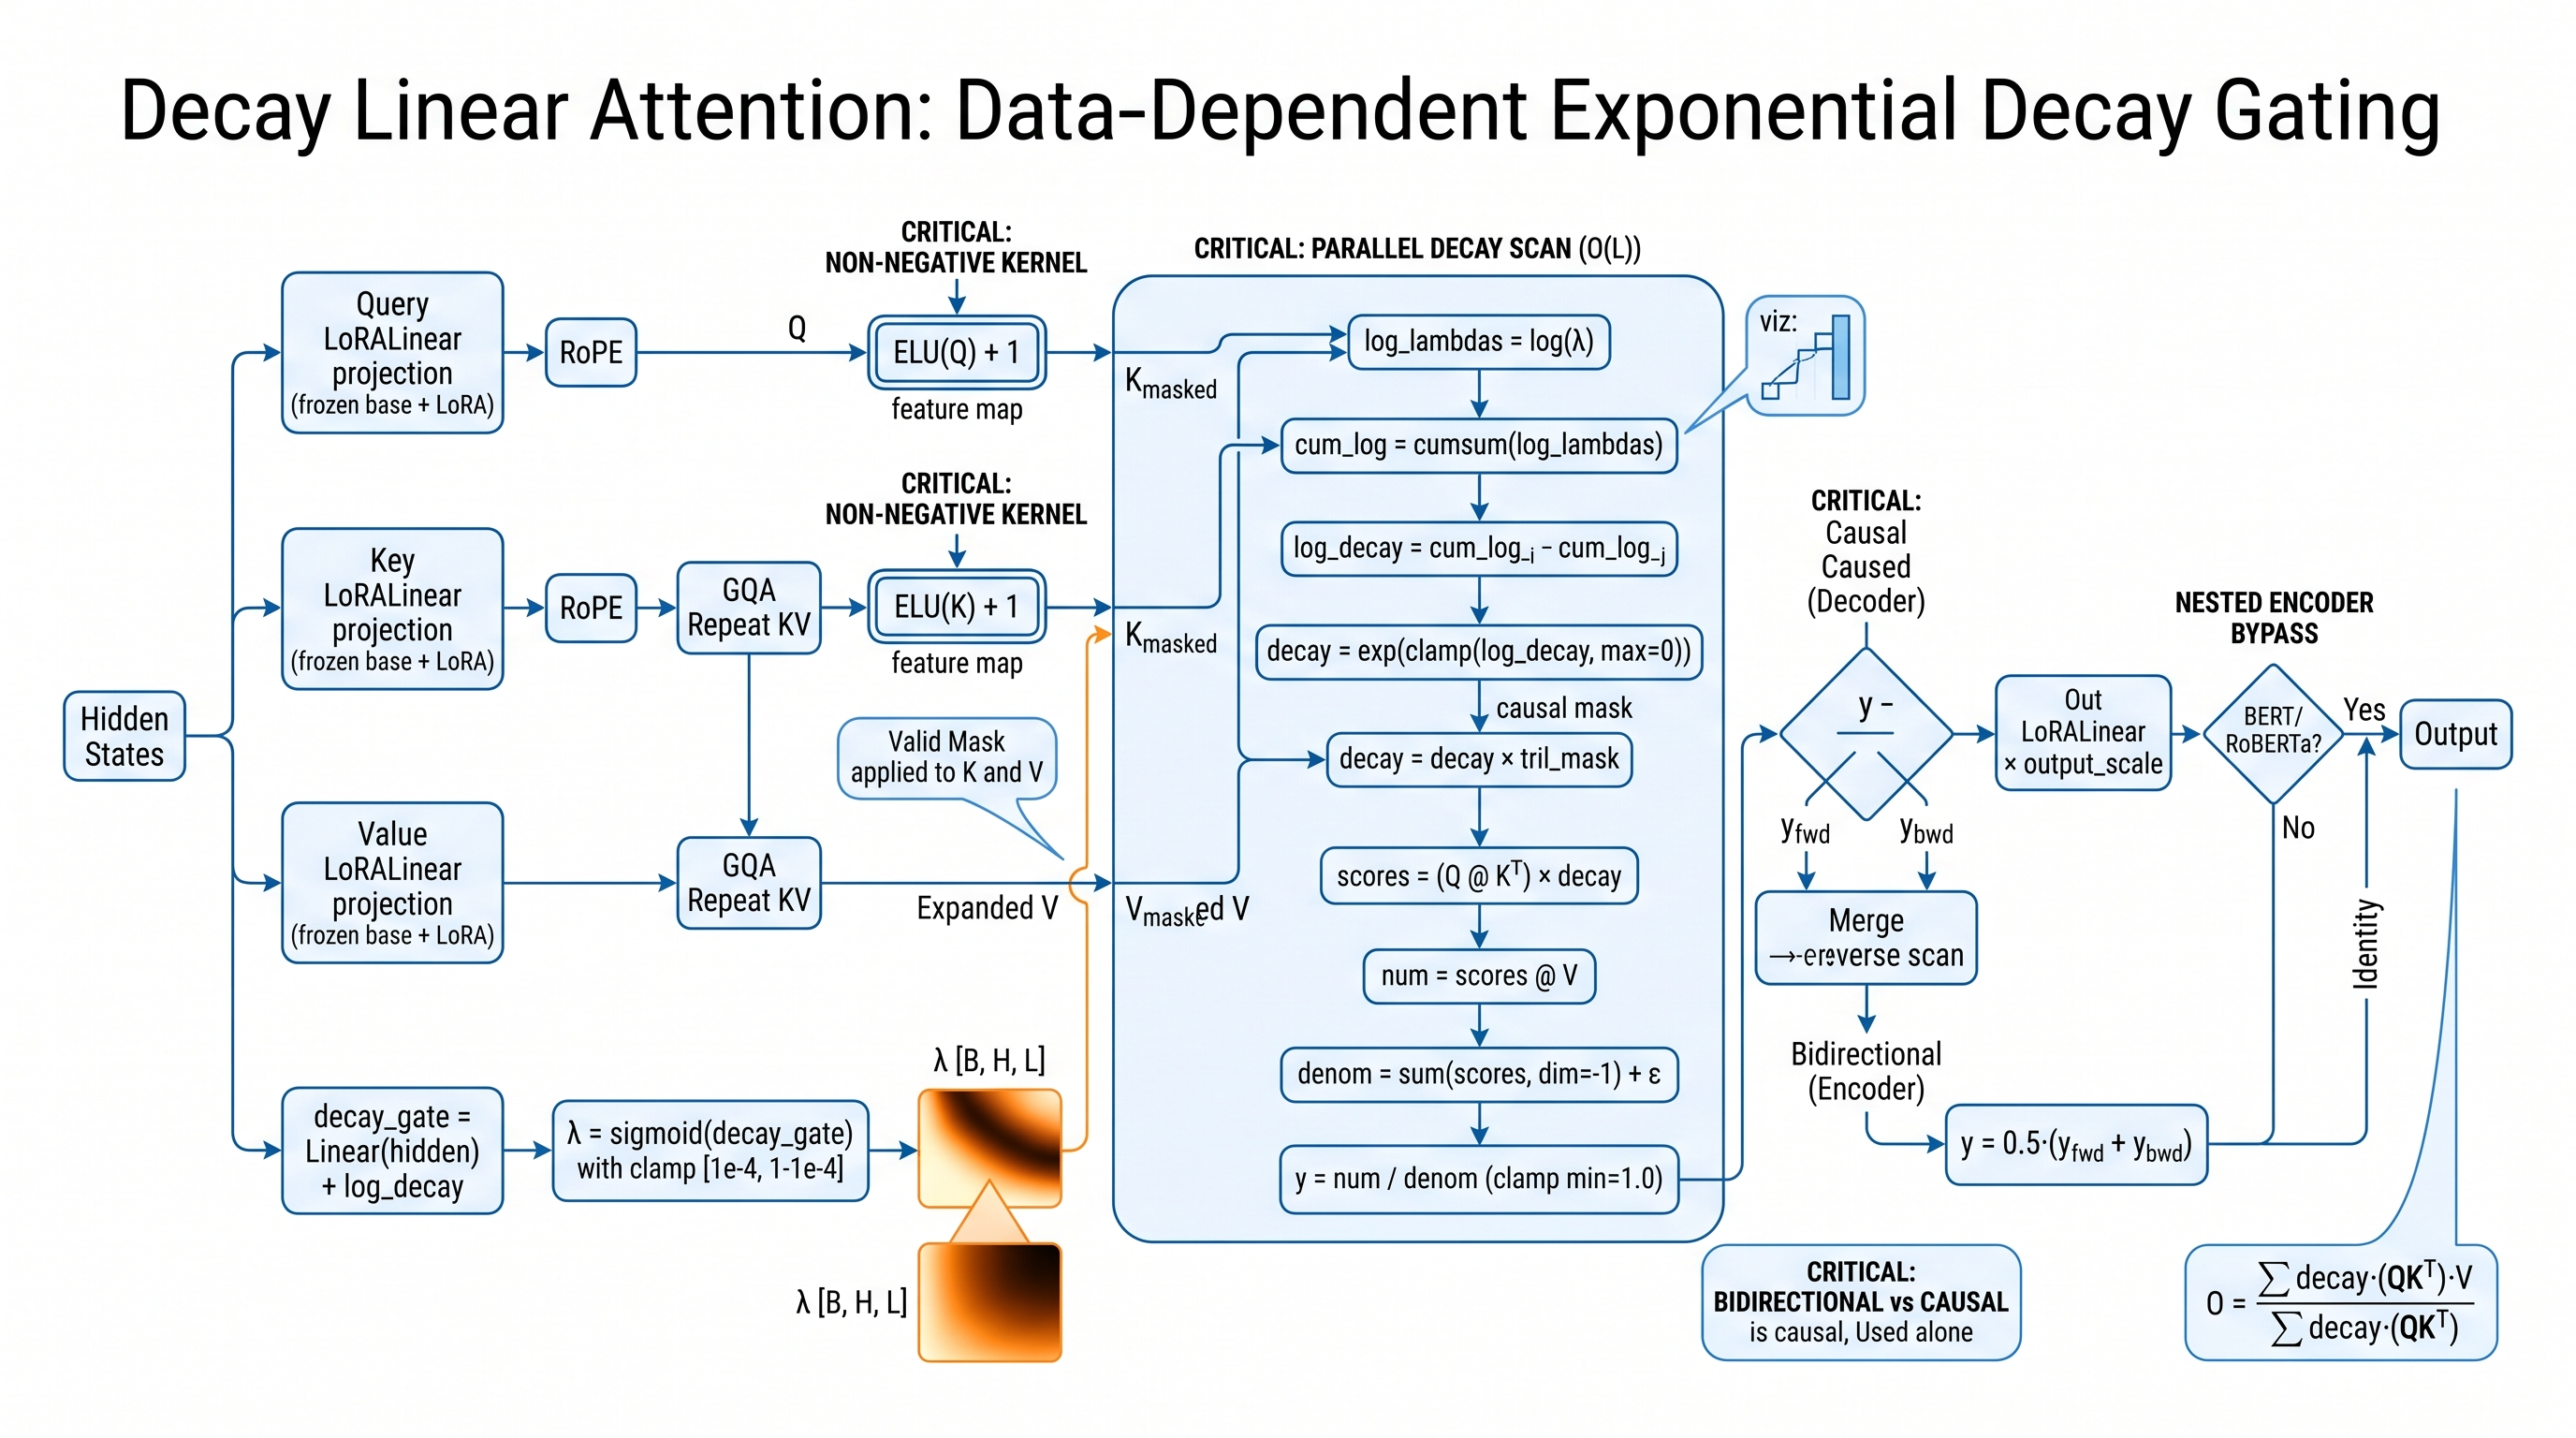
\includegraphics[width=\linewidth]{figures/architecture.jpeg}
\caption{High-level architectural diagram of decay\_linear\_attention.}
\label{fig:arch_decay-linear-attention}
\end{figure}

